\documentclass[12pt]{beamer}
\usetheme{Pittsburgh}
\usepackage[T1,T2A]{fontenc}
\usepackage[utf8]{inputenc}
\usepackage[bulgarian]{babel}
%\usepackage{amsmath}
%\usepackage{amsfonts}
%\usepackage{amssymb}
\usepackage{graphicx}

%\usepackage{enumerate}
%\usepackage{soul}


\title{Информационна система на агенция за недвижими имоти}
\subtitle{Част III: Информационен модел и UML диаграми}
\author{Екип $\pi \approx 3.1$}

%\setbeamercovered{transparent} 
\setbeamertemplate{navigation symbols}{} 
\date{} 

\begin{document}

\begin{frame}
\titlepage
\end{frame}

%\begin{frame}
%\tableofcontents
%\end{frame}

\begin{frame}[fragile]
\frametitle{UC Модел (1)}
        \begin{figure}[h]
        \centering
        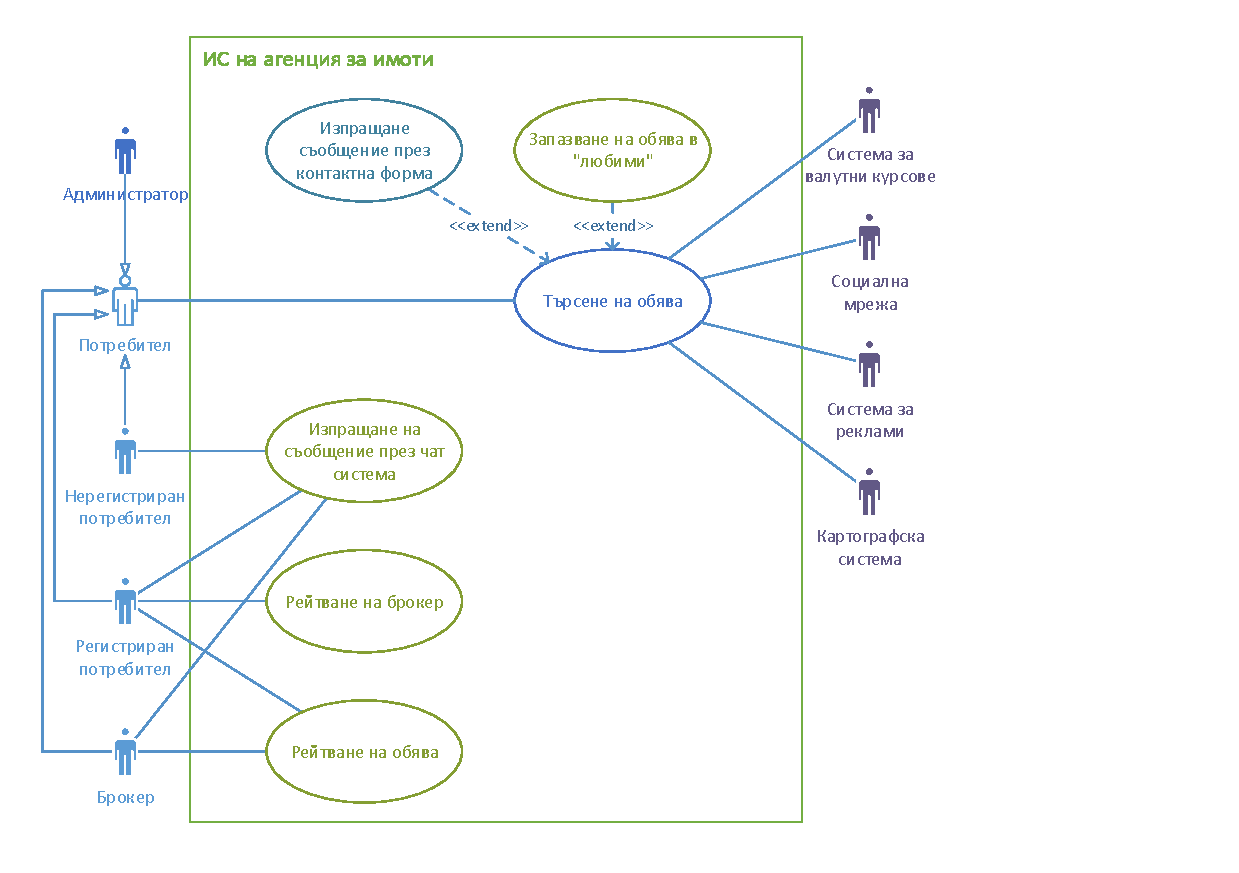
\includegraphics[scale=0.5]{uc2a}
        \end{figure}
\end{frame}

\begin{frame}[fragile]
\frametitle{UC Модел (2)}
        \begin{figure}[h]
        \centering
        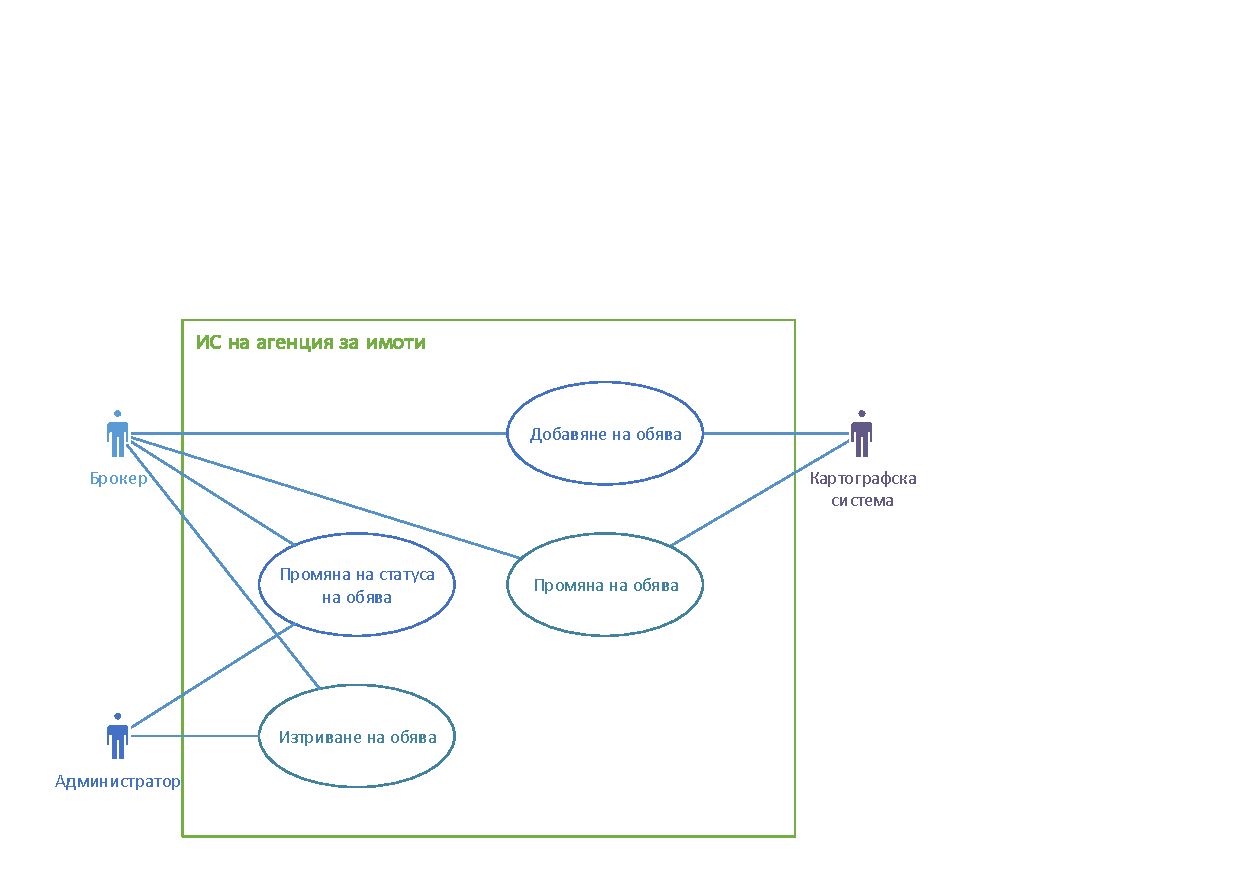
\includegraphics[scale=0.5]{uc2b}
        \end{figure}
\end{frame}

\begin{frame}[fragile]
\frametitle{UC Модел (3)}
        \begin{figure}[h]
        \centering
        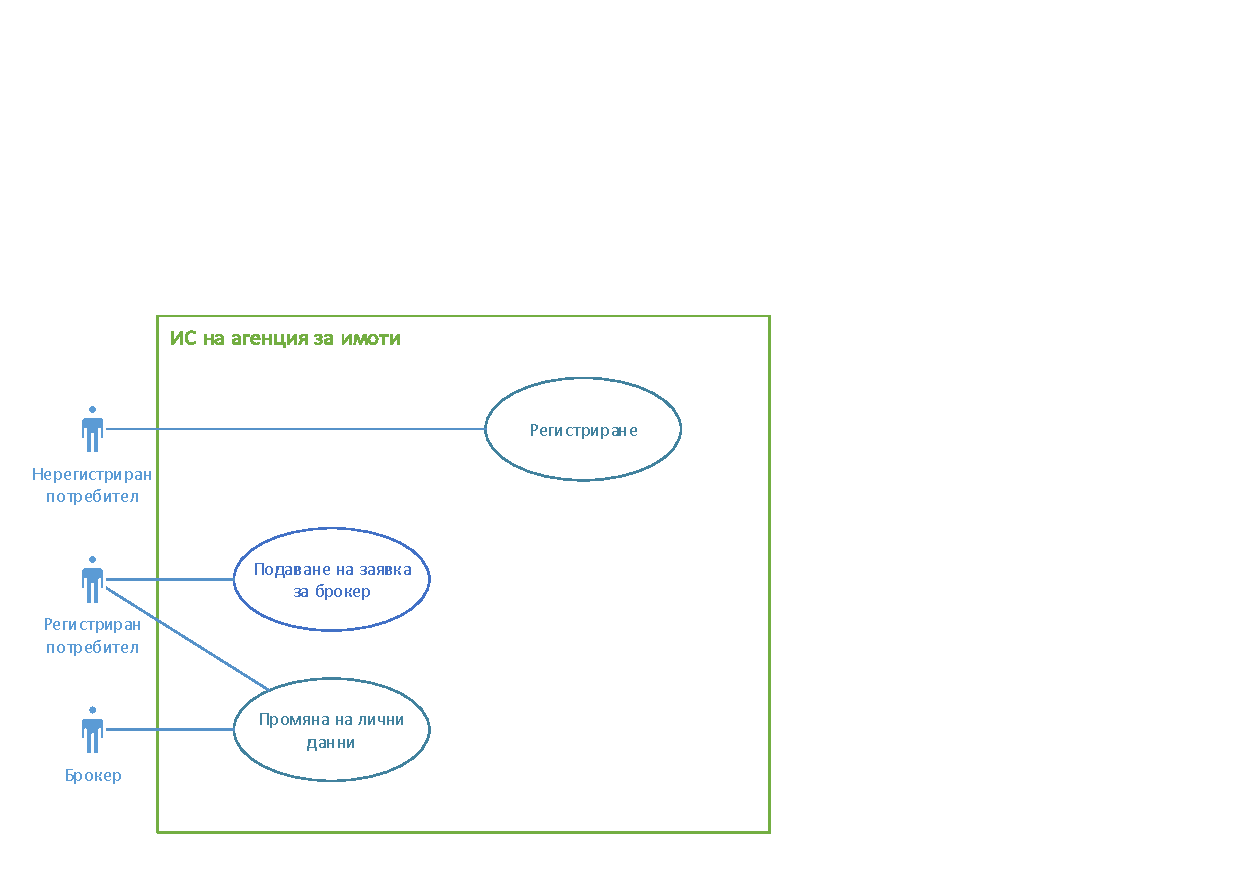
\includegraphics[scale=0.5]{uc2c}
        \end{figure}
\end{frame}

\begin{frame}[fragile]
\frametitle{UC Модел (4)}
        \begin{figure}[h]
        \centering
        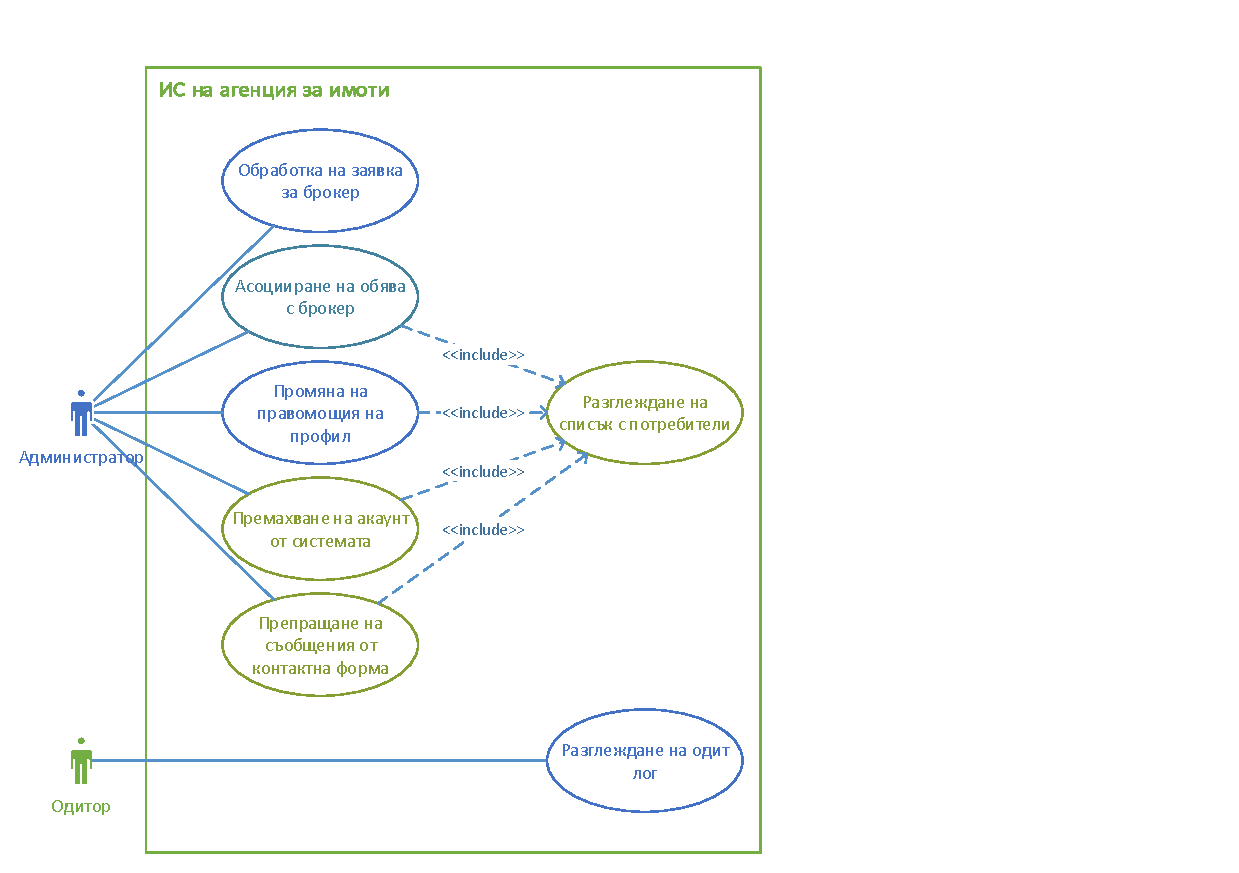
\includegraphics[scale=0.5]{uc2d}
        \end{figure}
\end{frame}

\begin{frame}[fragile]
\frametitle{Ред на реализация на UC (1)}
\begin{itemize}
\item C-7	Разглеждане на списък с потребители
\item A-5	Разглеждане на одит лог
\item B-2	Регистриране
\item B-3	Промяна на лични данни
\item A-6	Подаване на заявка за брокер
\item A-3	Обработка на заявка за брокер
\item A-2	Добавяне на обява
\item A-1	Търсене на обява
\item B-4	Промяна на обява
\item A-7	Промяна на статуса на обява
\item B-5	Изтриване на обява
\end{itemize}
\end{frame}

\begin{frame}[fragile]
\frametitle{Ред на реализация на UC (2)}
\begin{itemize}
\item B-6	Асоцииране на обява с брокер
\item A-4	Промяна на правомощия на профил
\item C-8	Премахване на акаунт от системата
\item B-1	Изпращане съобщение през контактна форма
\item C-6	Препращане на съобщения от контактна форма
\item C-3	Запазване на обява в ``любими''
\item C-4	Рейтване на обява
\item C-5	Рейтване на брокер
\item C-1	Споделяне на обява
\item C-2	Изпращане на съобщение през чат система
\end{itemize}
\end{frame}

\begin{frame}[fragile]
\frametitle{Домейн модел}
        \begin{figure}[h]
        \centering
		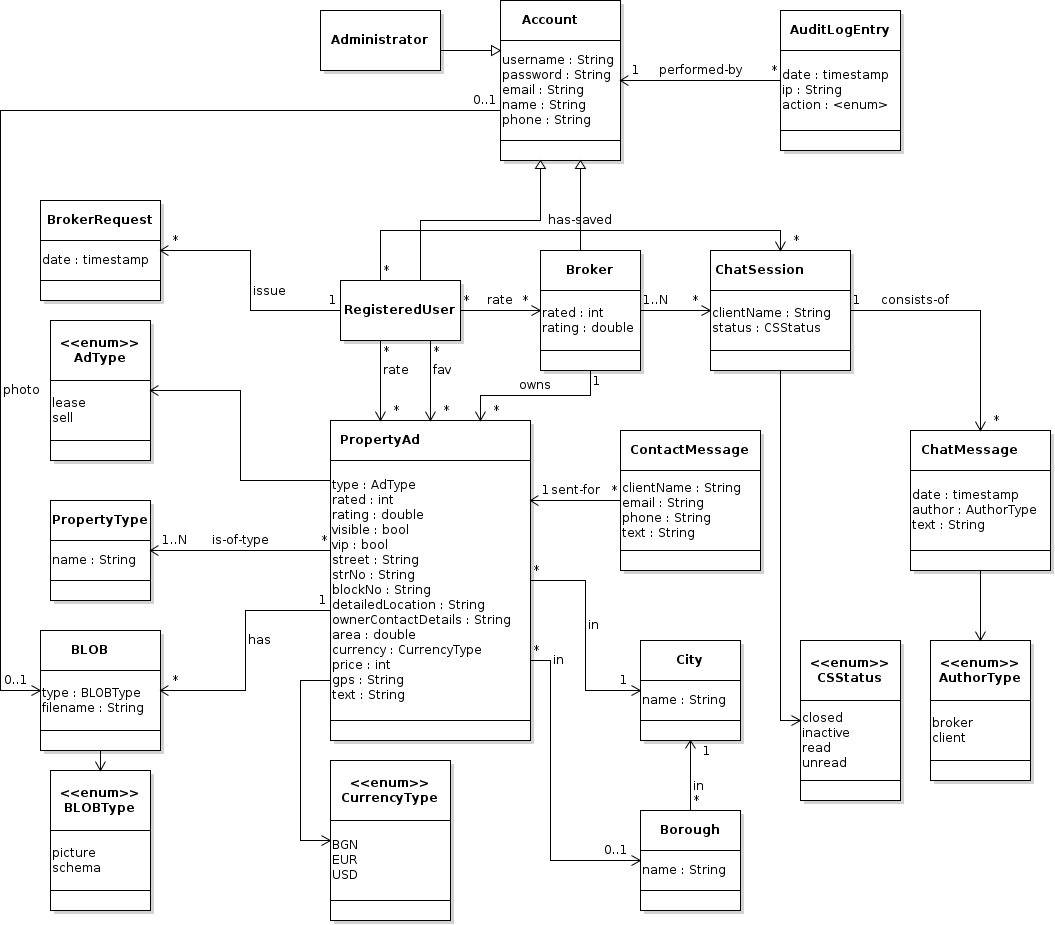
\includegraphics[scale=0.25,keepaspectratio=true]{domain-model}
        \end{figure}
\end{frame}

\begin{frame}[fragile]
\frametitle{Диаграма на комуникация за ``Търсене на обява''}
        \begin{figure}[h]
        \centering
		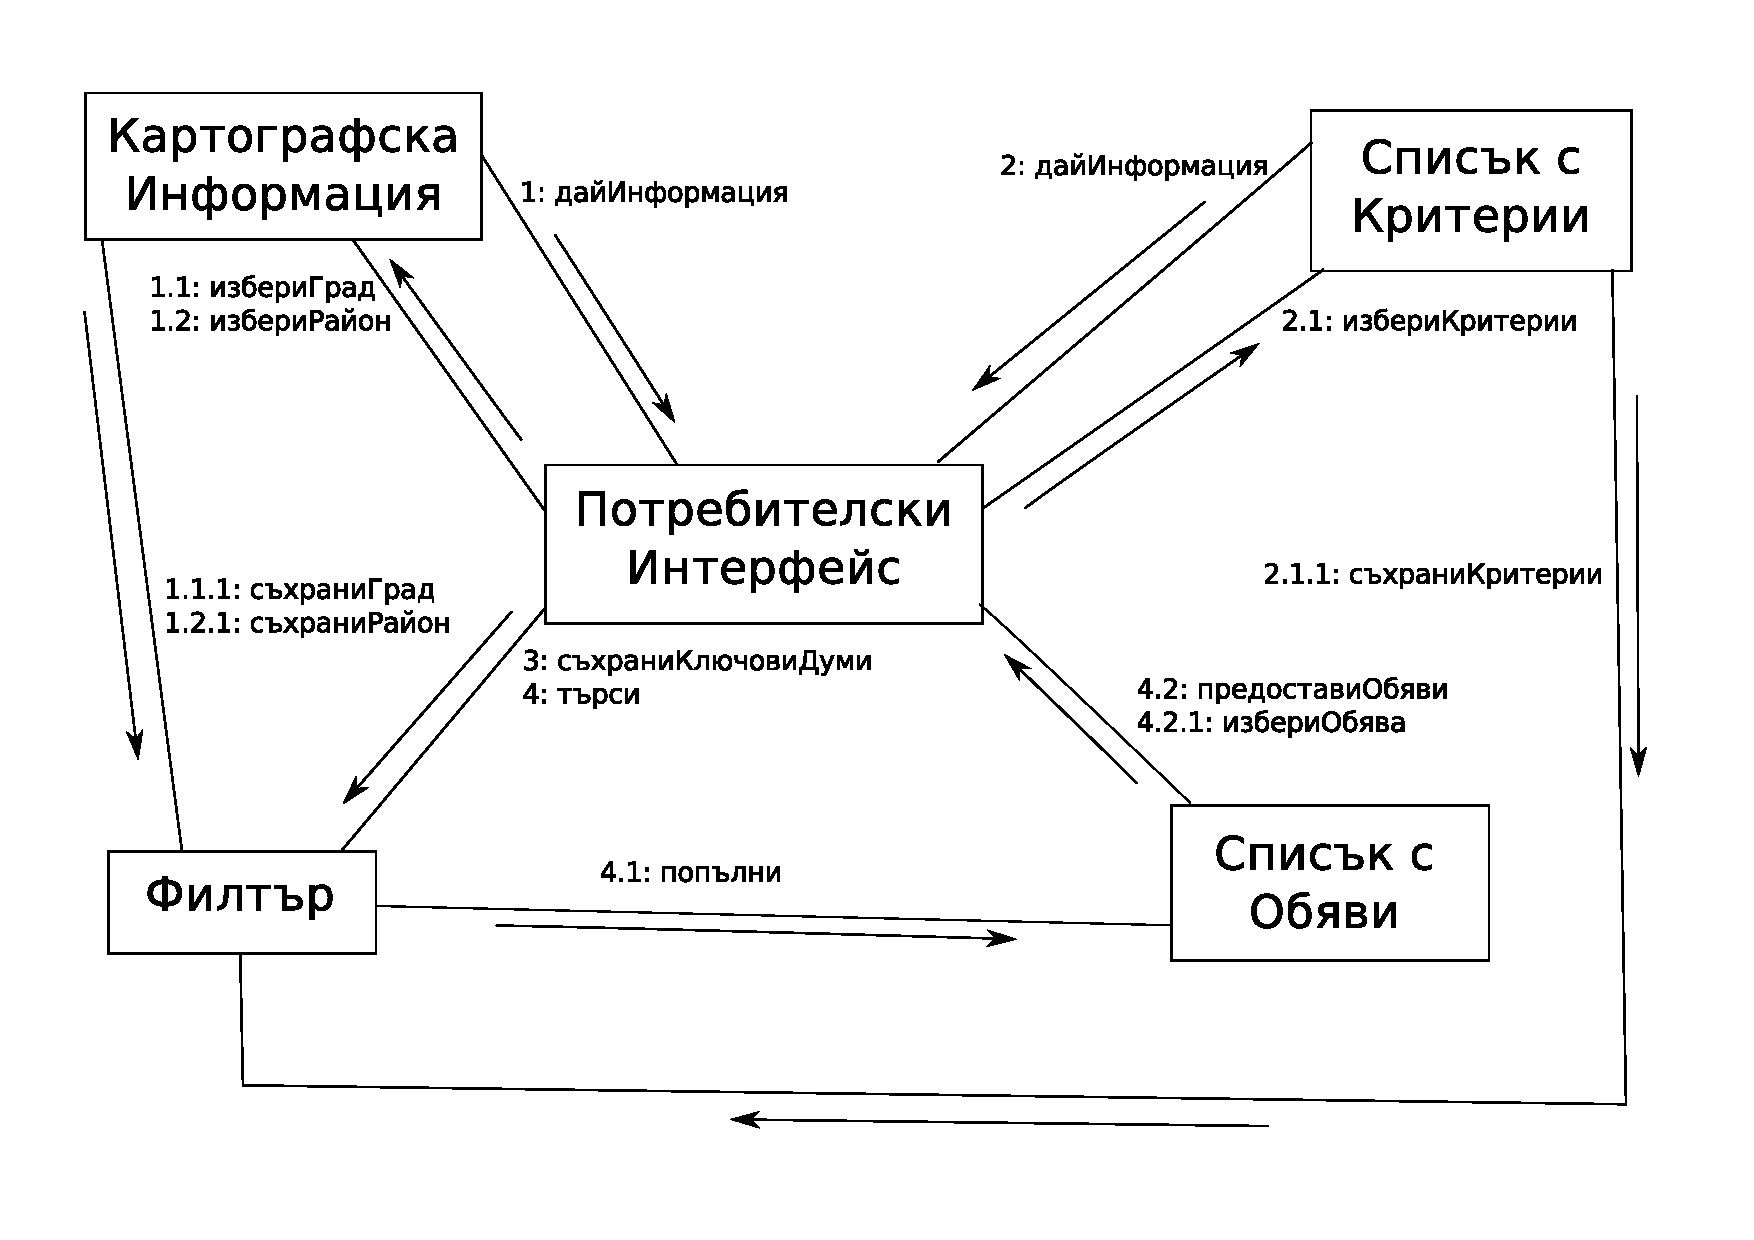
\includegraphics[scale=0.3,keepaspectratio=true]{uml02b}
        \end{figure}
\end{frame}

\begin{frame}[fragile]
\frametitle{Диаграма на дейността за ``Редактиране на обява''}
        \begin{figure}[h]
        \centering
		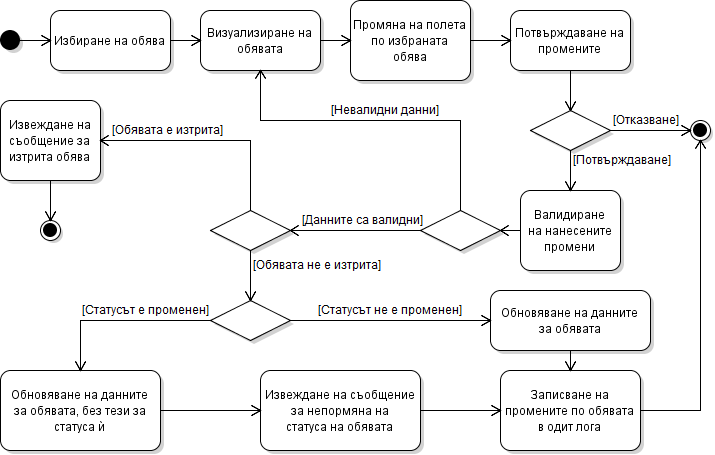
\includegraphics[scale=0.4,keepaspectratio=true]{uml3}
        \end{figure}
\end{frame}

\begin{frame}[fragile]
\frametitle{Диаграма на последователност за ``Получаване на права на брокер''}
        \begin{figure}[h]
        \centering
		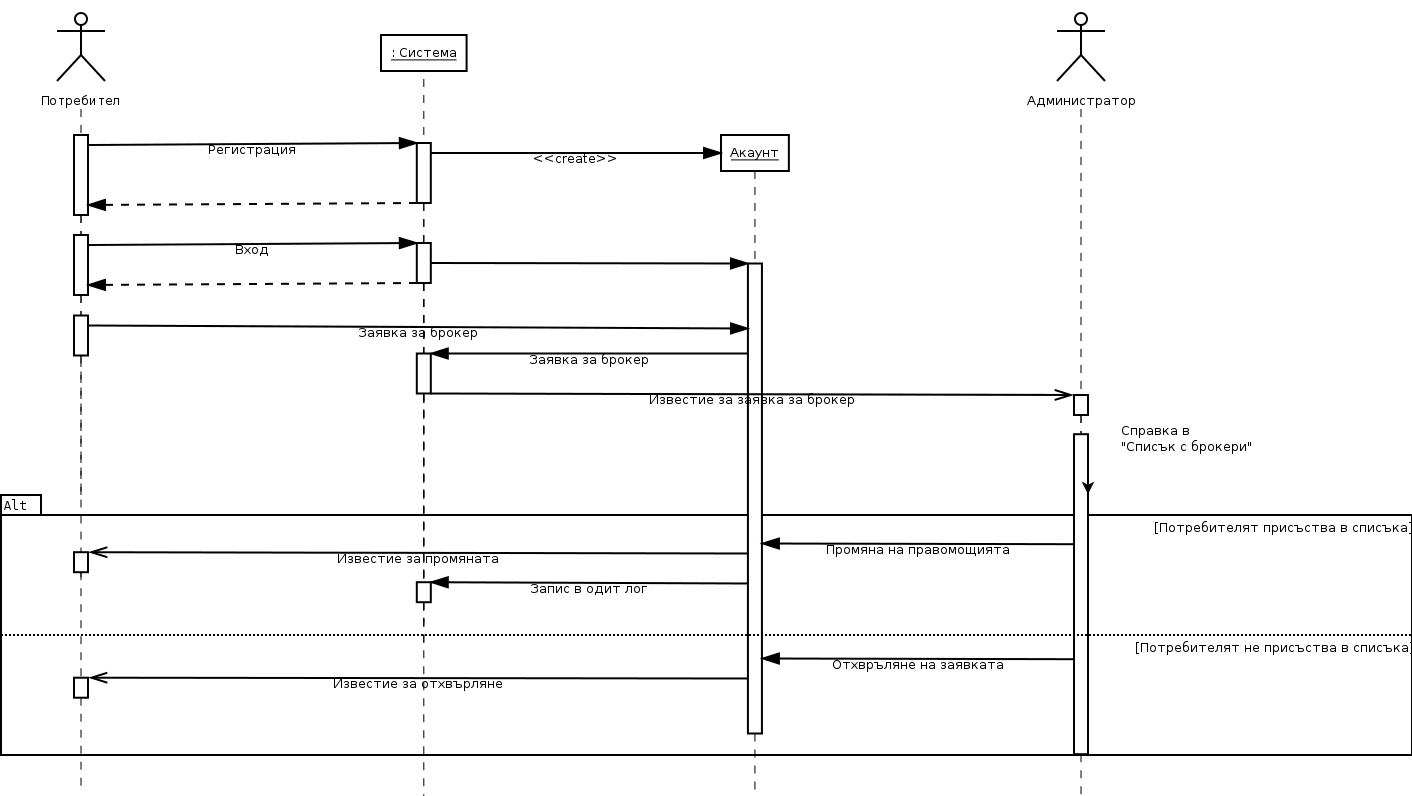
\includegraphics[scale=0.2,keepaspectratio=true]{uml04}
        \end{figure}
\end{frame}

\begin{frame}[fragile]
\frametitle{Диаграма на дейността за ``Обработка на заявка за брокер''}
        \begin{figure}[h]
        \centering
		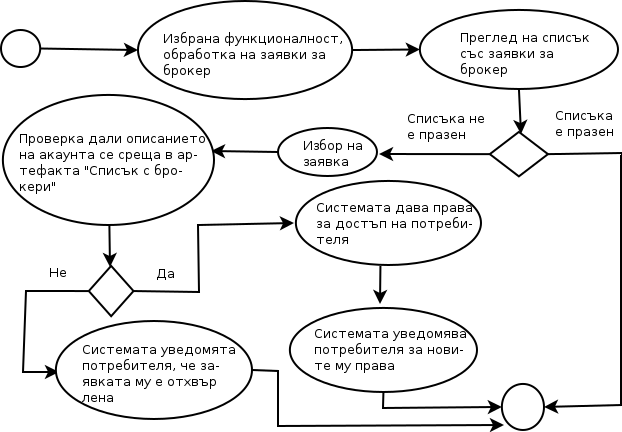
\includegraphics[scale=0.4,keepaspectratio=true]{uml06}
        \end{figure}
\end{frame}

\begin{frame}[fragile]
\frametitle{Диаграма на машина на състояние за ``Промяна на статуса на обява''}
        \begin{figure}[h]
        \centering
		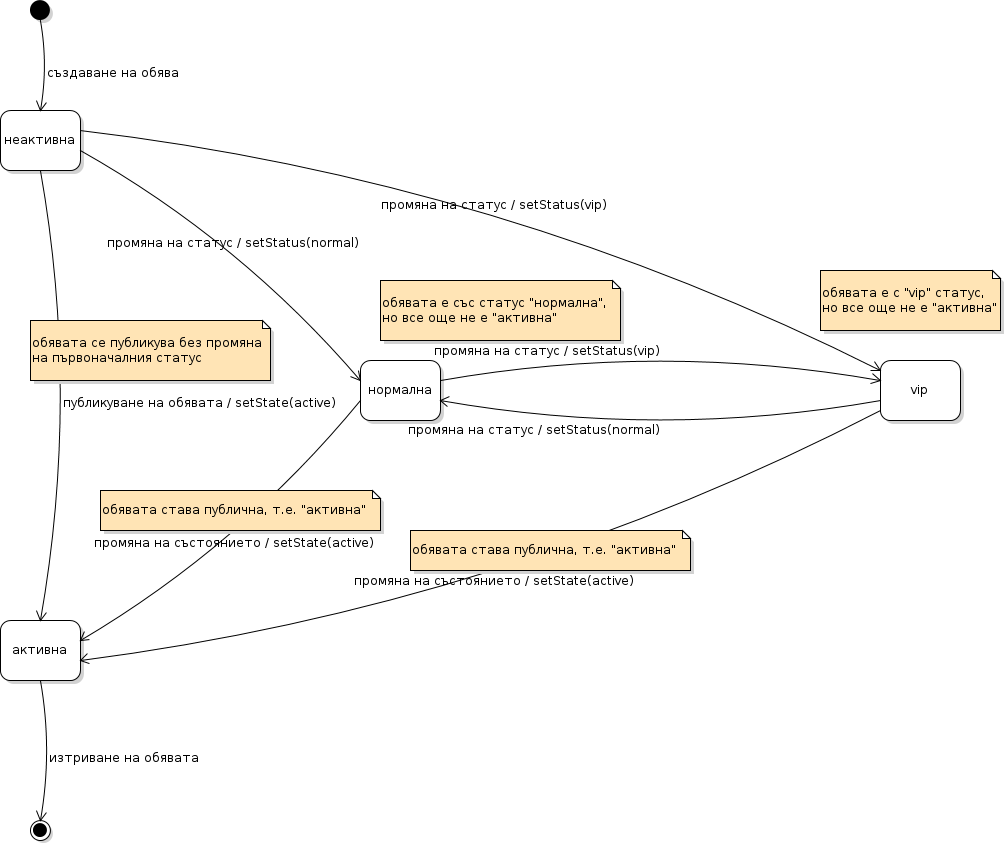
\includegraphics[scale=0.22,keepaspectratio=true]{uml07}
        \end{figure}
\end{frame}

\begin{frame}[fragile]
\frametitle{Диаграма на дейността за ``Изтриване на обява''}
        \begin{figure}[h]
        \centering
		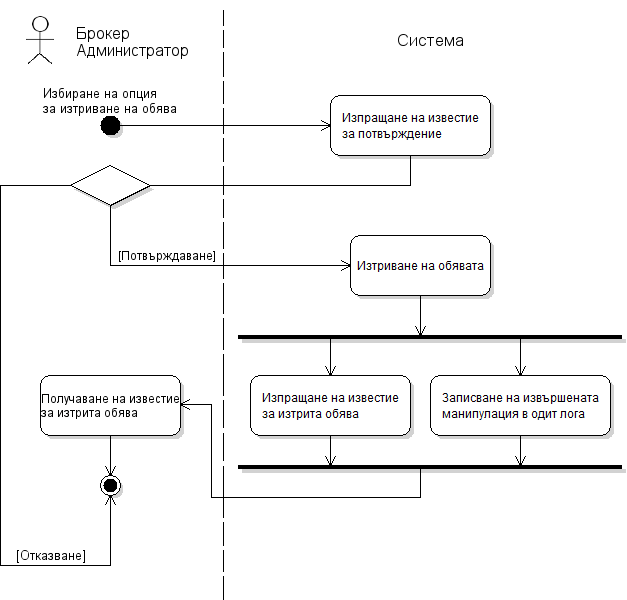
\includegraphics[scale=0.35,keepaspectratio=true]{uml08}
        \end{figure}
\end{frame}

\begin{frame}[fragile]
\frametitle{Диаграма на последователност за ``Добавяне на обява''}
        \begin{figure}[h]
        \centering
		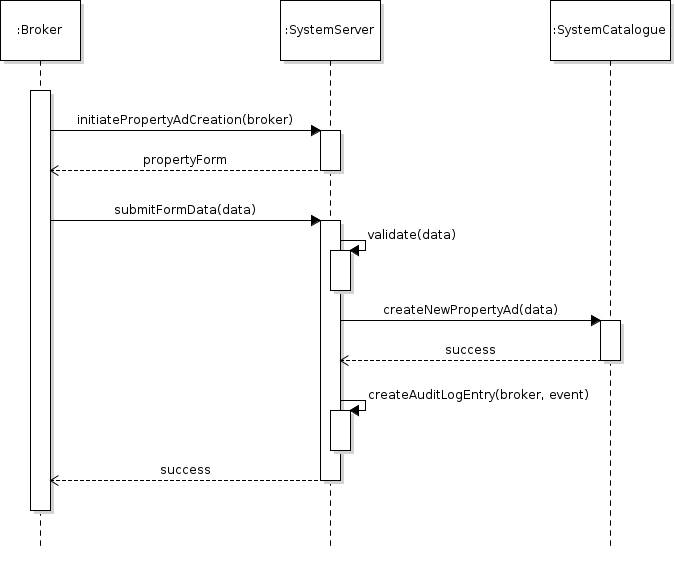
\includegraphics[scale=0.35,keepaspectratio=true]{uml09}
        \end{figure}
\end{frame}

\begin{frame}[fragile]
\frametitle{Диаграма на дейността за ``Отнемане на статус брокер''}
        \begin{figure}[h]
        \centering
		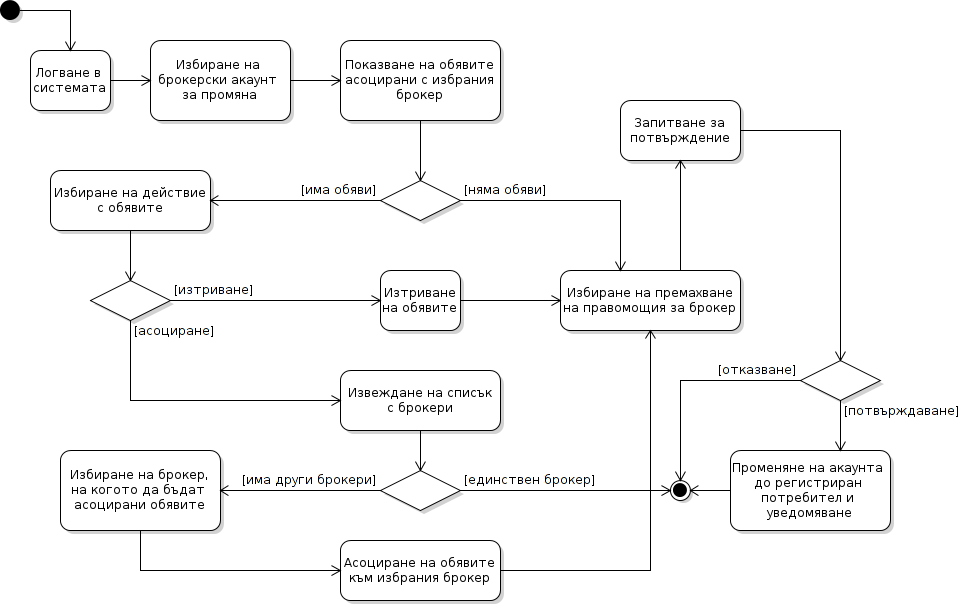
\includegraphics[scale=0.30,keepaspectratio=true]{uml10}
        \end{figure}
\end{frame}

\begin{frame}[fragile]
\frametitle{Примерен план на проекта (1)}
\begin{itemize}

\item {Планиране (Inception) (3w) %	10 (3w)
\begin{itemize}
\item Анализиране на изискванията (1w)
\item Дефиниране на функционалните и нефункционални изисквания (1w)
\item Формулиране на основните потребителски случаи (1w)
\end{itemize}
}
\end{itemize}
\end{frame}

\begin{frame}[fragile]
\frametitle{Примерен план на проекта (2)}
\begin{itemize}
\item {Детайлизиране (Elaboration) (7w) %	30 (7w)
\begin{itemize}
\item Обща системна архитектура (1w)
\item Детайлизиране на потребителските случаи (4w)
\item Проектиране на софтуерната архитектура (2w)
\end{itemize}
}
\end{itemize}
\end{frame}

\begin{frame}[fragile]
\frametitle{Примерен план на проекта (3)}
\begin{itemize}
\item {Изграждане (Construction) (15w) % 50 (15w)
\begin{itemize}
\item Завършване на дейностите по анализ и дизайн (1w)
\item Разработка на ядрото на системата (3w)
\item UC разработка и тестване, итерация 1 (1w)
\item UC разработка и тестване, итерация 2 (1w)
\item UC разработка и тестване, итерация 3 (3w)
\item UC разработка и тестване, итерация 4 (1w)
\item UC разработка и тестване, итерация 5 (1w)
\item UC разработка и тестване, итерация 6 (1w)
\item UC разработка и тестване, итерация 7 (2w)
\item Системни и интеграционни тестове (1w)
\end{itemize}
}

\end{itemize}
\end{frame}

\begin{frame}[fragile]
\frametitle{Примерен план на проекта (4)}
\begin{itemize}

\item {Предаване (Transition) (3w) % 10 (3w)
\begin{itemize}
	\item Внедряване при клиента (1w)
	\item Обучение на потребители (1w)
	\item Потребителски тестове (1w)
	\item Отстраняване на грешки
\end{itemize}
}
\end{itemize}
\end{frame}

\end{document}
